
\chapter[Estado del Arte]{Simulación de Materiales en Computación Gráfica: Estado del Arte}
\section{Introducción} %(hablar de los diferentes materiales, cómo los modelos "fáciles" no sirven)
El renderizado en computación gráfica es el intento de producir imágenes que representan una escena tridimensional, representada por medio de primitivas matemáticas como puntos, líneas, cubos, etc.

En los últimos años, el avance en el campo del renderizado de escenas ha sido muy notorio. El nivel de realismo presente en las imágenes obtenidas ha ido en aumento hasta el punto de ser de difícil distinción para un ser humano. Dichos avances han sido, en gran parte, debido al desarrollo de dispositivos de hardware gráficos más poderosos, ya que la teoría matemática que describe el comportamiento de la luz en escenas estuvo presente desde hace varias décadas mediante la denominada Ecuación del Renderizado \cite{Kajiya1986}.


La ecuación es una aproximación, un modelo físico que intenta describir los aspectos considerados más importantes en el fenómeno de interacción de la luz con diversos objetos en una escena.

Lamentablemente, la ecuación es, en términos teóricos, no computable. Sin embargo, el estudio a lo largo de los años de técnicas que permitan aproximarla ha dado sus frutos y ha permitido la obtención de imágenes de un realismo asombroso.

A pesar de estos increíbles avances en un corto período de tiempo, el renderizado de una escena es un problema que involucra otros inconvenientes. El más notorio de ellos, es que la ecuación del rendering no tiene en cuenta qué {\em materiales} componen los objetos que definen la escena. En otras palabras, un objeto compuesto por madera no lucirá exactamente igual que uno compuesto por metales, ni por un material orgánico compuesto de tejidos. A la par del desarrollo de técnicas de iluminación global, han surgido técnicas que han intentado abordar materiales específicos y familias de materiales.

Estas técnicas buscan capturar la intrincada geometría propia de cada material. Diferentes estructuras microscópicas producen distintas apariencias, reflejando la luz de distinta manera, hecho que es interpretado por la percepción humana como diferentes materiales. Por ejemplo: una superficie metálica tiene un gran componente reflexivo, emitiendo luz en direcciones bien definidas, a diferencia de una superficie más opaca como un plástico. Dado que la ecuación del renderizado usa los materiales como {\em caja negra}, los mismos deben ser modelados de una manera adecuada para ser integrados en las distintas técnicas de renderizado global.

Determinados materiales han recibido mayor atención debido a su ubicuidad en escenas de películas y video juegos, o a la facilidad de su diseño: agua, fuego, aire, humo, piel humana, madera, etc. Por esta razón, las imágenes sintéticas obtenidas presentan cierta asimetría en la calidad de los distintos materiales. En contraste, otros materiales han recibido menor atención, la cual puede atribuirse a una menor presencia en escenas o a una dificultad en el modelado y visualización, la cual ha resistido las técnicas más simples.

Entre estos materiales, aquellos sometidos a un proceso de cocción han permanecido entre los más dificultosos por su compleja geometría y los fenómenos lumínicos involucrados. Tal vez el caso más emblemático de los materiales cocidos es el pan, debido a su importancia en la vida cotidiana. Como nota de color, un reconocido  científico del área, Alain Fournier, pronunció en 2001 la frase "la Computación Gráfica todavía no ha sido capaz de renderizar de manera convincente una feta de pan". En las siguientes secciones mostraremos que unos pocos intentos por abordar el problema fueron realizados pocos años después.

\section{Modelos de Geometría de Materiales}
En esta sección presentaremos distintos modelos geométricos que han hecho su aparición a lo largo de los años en computación gráfica.
Los mismos son el resultado de un balance entre detalle de representación, tiempos de cómputo y recursos de memoria utilizados.
Casi en todos los materiales en computación gráfica, un modelo de geometría correcto es necesario para lograr imágenes realistas de los materiales a ser renderizados.

\subsection{Modelos Procedimentales}
Un modelo procedimental resulta útil en determinadas situaciones donde la supervisión humana repetitiva no es adecuada.

Existen numerosos ejemplos donde se aplica una técnica de modelado procedimental.
En las siguientes sub-secciones presentaremos los casos más comunes de aplicación, los cuales constituyen estándares actuales en el modelado de dichos materiales.
Si bien los resultados obtenidos presentan un gran realismo, los modelos utilizados no tienen una base física, por lo cual luego se muestra un ejemplo de la utilización de modelos físicos para el diseño de materiales.


\subsection{Plantas}
El modelado procedimental de plantas está basado en una interpretación de una tortuga que se mueve por un plano o el espacio, construyendo la geometría de los materiales \cite{Prusinkiewicz1986}.

Las gramáticas formales \cite{Chomsky1956} intentaron describir el lenguaje natural de forma matemática, donde sub-cadenas de caracteres son reemplazadas por otras.
Siguiendo esta idea, los sistemas-L \cite{Lindenmayer1968} pretenden realizar una descripción matemática de la geometría de las plantas.
El concepto central que permite entender el modelado procedimental utilizando sistemas-L es el de {\em reescritura}.
La reescritura consiste en una aplicación sucesiva de reglas que reemplazan determinadas partes en una descripción matemática por otras.
En un sistema-L, una cadena de caracteres representa la estructura de la planta.

\subsubsection{Definición de sistema-L}
Sea $V$ un alfabeto (conjunto de caracteres), $V^{*}$ el conjunto de todas las palabras que se pueden formar con $V$ y $V^{+}$ el conjunto de todas las palabras que se pueden formar y no son vacías.
Una sistema-L de cadenas es una tripleta $G = (V,\omega,P)$, donde $V$ es el alfabeto, $\omega \in V^{+}$ es una cadena no vacía llamada {\em axioma} y $P \subset V \times V^{*}$ es un conjunto finito de reglas de producción.
Una producción $(a,\chi)$ se denota $a \rightarrow \chi$.
$a$ es llamado el {\em predecesor} y $\chi$ el {\em sucesor} de la producción.
Si no se especifica ninguna producción para $a$, se asume $a \rightarrow a \in P$.

Sea $\mu = a_{1}, \dots, a_{m}$ una palabra en $V$.
Se dice que la palabra $\mu_{1}, \dots, \mu_{m}$ es {\em derivada directamente} de $\mu$, y se nota $\mu \Rightarrow \eta$,  si y sólo si $a_{i} \rightarrow \mu_{i}, \forall i = 1, \dots, m$.

Una palabra $\eta$ es generada por $G$ si existe una secuencia de cadenas que conducen a $\eta$ desde el axioma, es decir, $\mu_{1},\dots,\mu_{n}$, de tal forma que $\mu_{1} = \omega$ y $\mu_{n} = \eta$ y $\mu_{1} \Rightarrow \dots  \Rightarrow \mu_{n}$.

Un ejemplo de esto es expuesto a continuación.
Si el axioma es $\omega = a$, y las reglas de producción son:
\begin{align*}
p1 &: a \rightarrow b,\\
p2 &: b \rightarrow ab,
\end{align*}

entonces una cadena de derivaciones podría resultar $a, b, ab, bb, abab, \dots$, donde las reglas aplicadas en cada paso serían $p1, p2, p1, p2$ (dos veces).

Estos sistemas fueron diseñados buscando representar las divisiones celulares existentes en ciertas amebas.
Sin embargo, luego se mostrará que los mismos pueden ser utilizados como modelos para capturar la geometría de diversos objetos.

\subsubsection{Interpretación de Tortuga}
El estado de la tortuga se define por una tripleta $(x,y,\alpha)$, donde $x,y$ representan la posición de la tortuga y $\alpha$ es el ángulo hacia donde {\em apunta} la tortuga.
Dado un tamaño de paso $d$ y un incremento angular de $\delta$, la tortuga puede "programarse" para responder a cadenas de caracteres con la siguiente interpretación,

\begin{itemize}
\item F, moverse hacia adelante un paso d, dibujando,
\item f, moverse hacia adelante un paso d, sin dibujar,
\item +, rotar un ángulo $\delta$,
\item -, rotar un ángulo $-\delta$.
\end{itemize}

Al interpretarse el comando $F$, el nuevo estado de la tortuga será $(x',y',\alpha)$, donde $x' = x + d * cos(\alpha)$ y $y' = y + d * sin(\alpha)$. Se dibuja además una línea entre $(x,y)$ y $(x',y')$.
Al interpretarse el comando $f$ ocurre lo mismo, sólo que la línea no se dibuja.
Cuando se lee el comando $+$ (girar a la izquierda). el nuevo estado pasa a ser $(x,y,\alpha-\delta)$ y cuando se interpreta $-$ (girar a la derecha),  $(x,y,\alpha+\delta)$.

De esta forma, dada una cadena $\eta$, la interpretación de tortuga de la misma es la imagen que se genera al responder la tortuga a los comandos inducidos por $\eta$.
La Fig.~\ref{fg:tortuga} muestra un ejemplo de la figura resultante de la cadena FFF-FF-F-F+F+FF-F-FFF, donde la tortuga comienza {\em mirando} hacia arriba, y $\delta = 90^{\circ}$.

\begin{figure}
\center
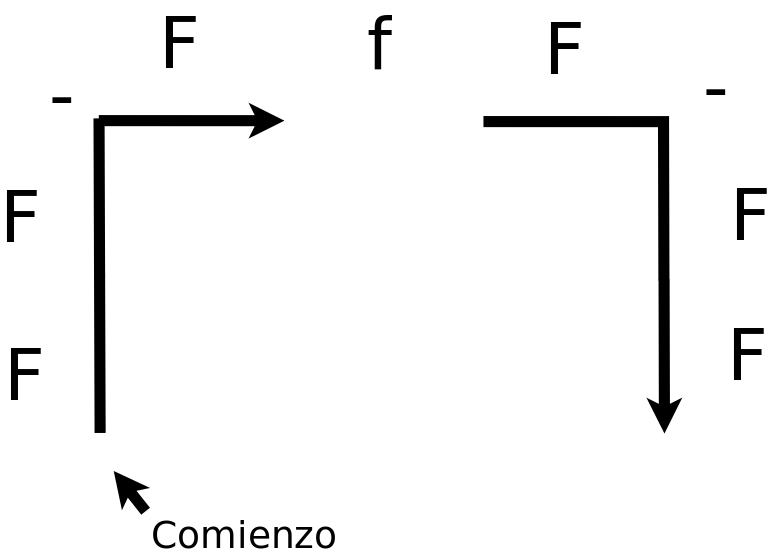
\includegraphics[width=8cm]{figures/tortuga}
\caption{Resultado de la interpretación de tortuga de una cadena de caracteres.}
\label{fg:tortuga}
\end{figure}

La Fig.~\ref{fg:tortuga} muestra otros ejemplos de sistemas-L, en los cuales se puede observar que con pocas reglas es posible obtener estructuras complejas y de gran belleza.

Usualmente, y debido a la utlización de recursión y repetición, estos sistemas dan lugar a figuras fractales, por lo cual se las utiliza para dibujar este tipo de estructuras autosimilares.

\begin{figure}
\center
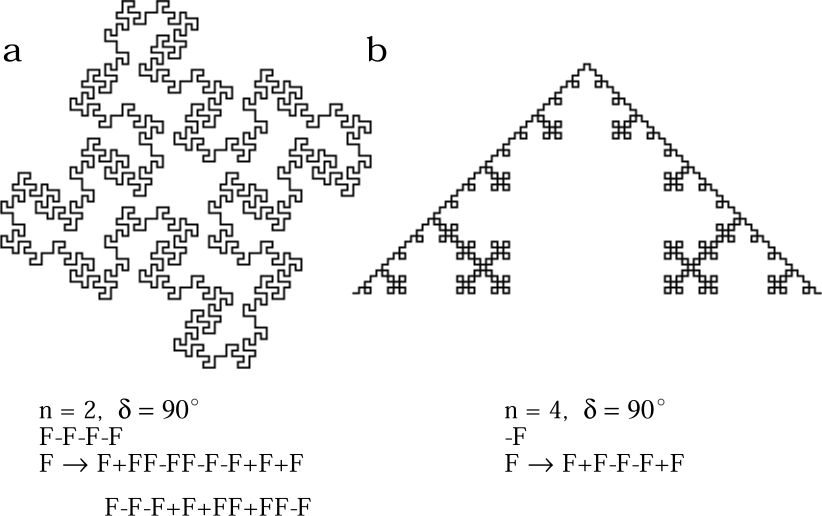
\includegraphics[width=13cm]{figures/sistemasL}
\caption{Sistemas-L generados utilizando distintos parámetros. $n$ es la cantidad de derivaciones utilizadas para producir la cadena que da origen a la figura. En (a), el axioma es F-F-F-F, mientras que en (b) es -F.}
\label{fg:sistemasL}
\end{figure}

Para lograr una imagen que semeje la estructura de árboles y plantas, es necesario introducir dos nuevos caracteres, los cuales son utilizados para generar estructuras ramificadas.
Utilizando una {\em pila} de estados, es posible alcanzar este comportamiento.
Los caracteres $[$, y $]$ se utilizan para mover el estado actual a la pila, y para reemplazar el estado actual con el de la pila, respectivamente.
El estado actual de la tortuga está representado por la tripleta antes mencionada.
Por lo tanto, al realizar la operación $]$, en general la posición y orientación de la tortuga cambiarán.
La utilización de un par $[\dots]$ produce que la tortuga dibuje una rama y vuelva al punto inicial, permitiendo continuar con la computación de otras partes de la estructura.

\begin{figure}
\center
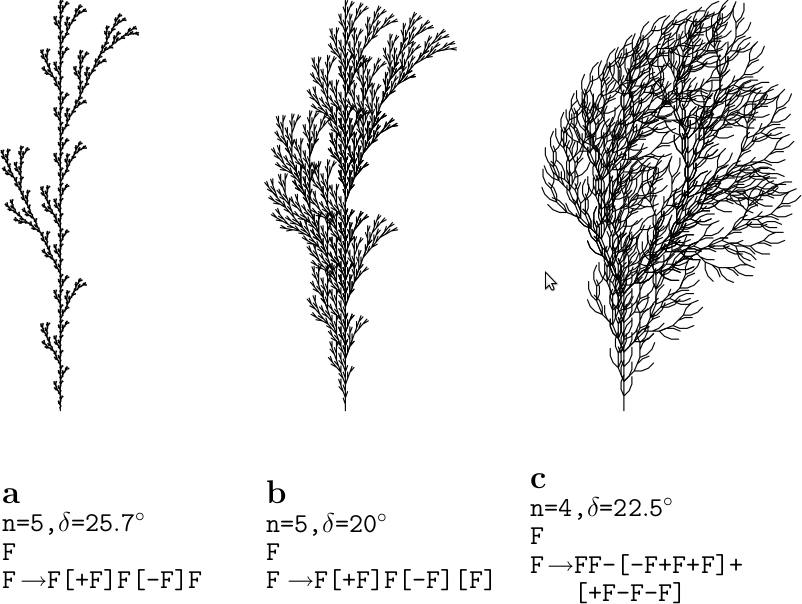
\includegraphics[width=13cm]{figures/sistemalcorchete}
\caption{Sistemas-L con pila de estados, utilizando distintos parámetros. Las imágenes muestran estructuras muy parecidas a plantas. $n$ es la cantidad de derivaciones utilizadas para producir la cadena que da origen a la figura.}
\label{fg:sistemasLcorchete}
\end{figure}


Existen numerosas variantes a estos sistemas, entre los cuales encontramos sistemas-L estocásticos, los cuales eligen reglas de reescritura de acuerdo a una probabilidad que se pasa como parámetro, sistemas-L paramétricos, los cuales hacen variar el ángulo y el paso a dibujar dependiendo de la posición de la cadena donde se encuentran, y muchos otros.
Además, el método es fácilmente generalizable en tres dimensiones, ver \cite{Prusinkiewicz1990} para obtener mayores detalles.

\subsection{Edificios y Ciudades}
Una de las ventajas del modelado procedimental es la capacidad de realizar el proceso prácticamente sin intervención humana, ahorrando costos y tiempos de diseño.
En esta línea se ubica el trabajo de \cite{Wonka2003}, donde un proceso automático genera, de manera casi instantánea, edificios arquitectónicamente coherentes, es decir, con ciertas características estructurales que deben ser respetadas.

La diferencia principal a la hora de utilizar sistemas-L para modelar edificios, es que los mismos no pueden ser modelados como una estructura que crece, sino que deben tratarse como conjuntos de objetos con una disposición específica.

Para lograr esto, en \cite{Wonka2003} se proponen varias definiciones, entre las que se encuentran gramáticas de división y gramáticas de control.

Una {\em forma} es un conjunto de líneas rectas en el espacio.
Las gramáticas de división seleccionan reglas para subdividir formas en formas más básicas (cubos, cilindros, etc.).


Una gramática puede ser definida de manera general como un álgebra de objetos $(U,+,-,F,\leq)$, cerrada bajo las operaciones $+$ y $-$, junto a un conjunto de operaciones $F$, de tal forma que si $u$ y $v$ son miembros de $U$, entonces $u+f(v)$ y $u-f(v)$ lo son, donde $f \in F$.
Una gramática $G=(N,T,R,I)$ es una tupla que consta de cuatro elementos, donde $N \subset U$ representa los nodos no terminales, $T \subset U$ los terminales, $I \subset N$ un conjunto de objetos iniciales y un conjunto de producciones $R \subseteq U \times U$.

%Para comprender mejor estos conceptos, definimos una gramática de conjuntos.
%Este tipo de gramáticas 

La Fig.~\ref{fg:splitgrammar} muestra un ejemplo del proceso involucrado en una gramática {\em de división}, en la cual una {\em forma} es dividida en otras, utilizando reglas definidas por dicha gramática, en este caso formando una secuencia de ventanas.
Como puede observarse, una gramática de este tipo divide de forma completa el espacio de las formas padre, en formas hijas de la misma.

Cuando el proceso llega a su fin, es decir, no existen nodos no terminales ($N$) en el desarrollo, entonces lo que se tiene es un {\em diseño} final.
La principal diferencia con los sistemas-L se basa en que en aquellos, las reescrituras no necesariamente ocupaban el mismo volumen, como sí debe ocurrir en estas gramáticas.

\begin{figure}
\center
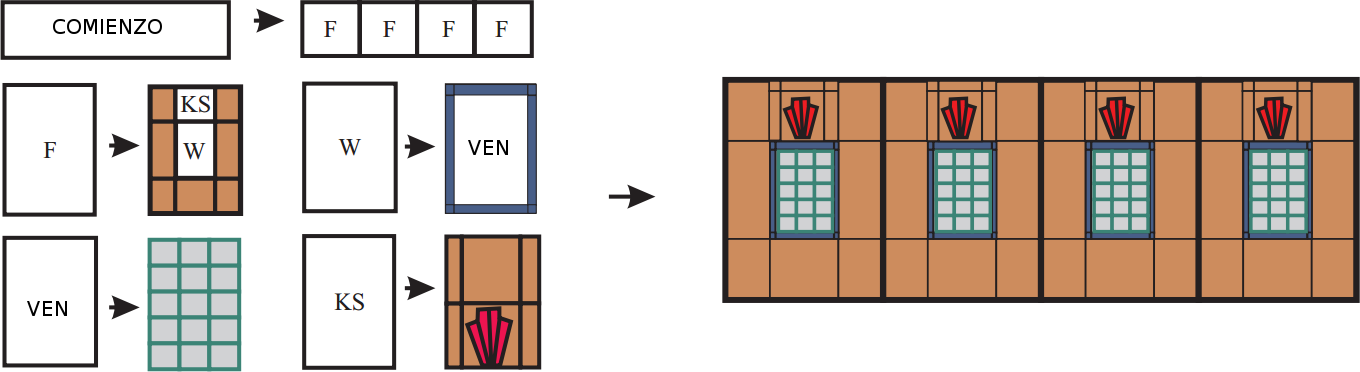
\includegraphics[width=13cm]{figures/splitgrammar}
\caption{Gramática de división mostrando los pasos seguidos para formar una secuencia de ventanas.}
\label{fg:splitgrammar}
\end{figure}

Por otro lado, las gramáticas de control permiten tomar decisiones de diferenciación sobre las divisiones, con la idea de generar al mismo tiempo aleatoriedad en los edificios resultantes.
Por ejemplo, se puede querer que la apariencia del primer piso de un edificio sea diferente al resto (puertas).
La Fig.~\ref{fg:controlgrammar} muestra un ejemplo de una gramática de control.

Las texturas, colores y otras decisiones pueden controlarse por medio de {\em atributos}.
Esto resulta útil para mantener la coherencia en un mismo piso, por ejemplo, o asegurar que todas las columnas del edificio seguirán un mismo diseño arquitectónico.
Los nodos terminales de la gramática presentan datos de posicionamiento con la forma $(c,a,v)$, donde $c$ es la posición en la división (fila, columna, capa, en $3D$), $a$ es el atributo y $v$ el valor que tomará.
Las gramáticas de control también cumplen el propósito de lograr una distribución correcta de las formas.
Por medio de ellas, es posible {\em excluir} elementos de ciertas posiciones indeseadas (por ejemplo una puerta en el tercer piso), utilizando los mismos atributos para elegir determinadas reglas por sobre otras, logrando coherencia y balance de formas en los resultados finales.

\begin{figure}
\center
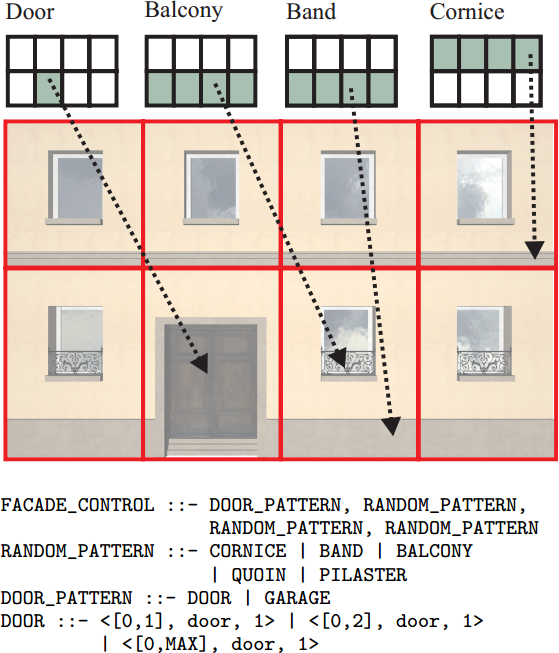
\includegraphics[width=11cm]{figures/controlgrammar}
\caption{Gramática de control.}
\label{fg:controlgrammar}
\end{figure}

La literatura de modelado procedimental de edificios y ciudades está creciendo en los últimos años \cite{Parish2001,Muller2006}.
La Fig.~\ref{fg:edificios} muestra ejemplos de edificios generados procedimentalmente.



\begin{figure}
\center
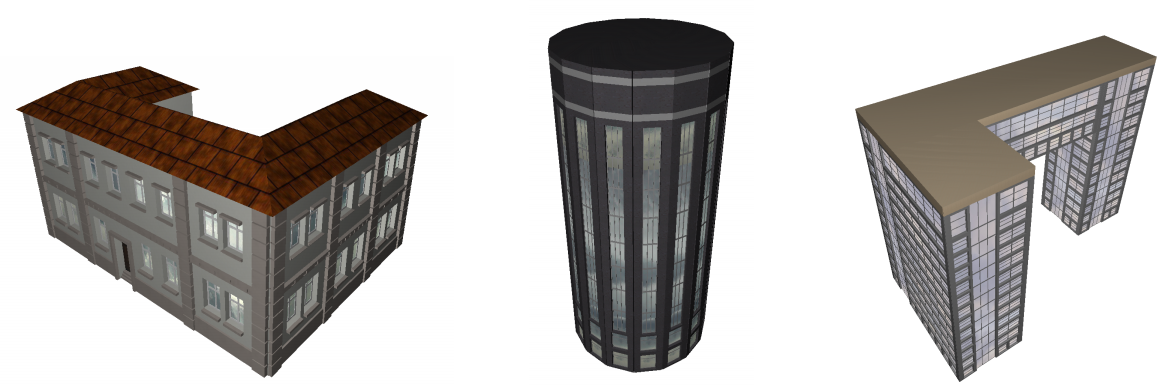
\includegraphics[width=11cm]{figures/edificios}
\caption{Edificios generados procedimentalmente por medio de gramáticas.}
\label{fg:edificios}
\end{figure}

\subsection{Fractales y Montañas}
Una forma particularmente interesante de modelar fenómenos de apariencia pseudo-aleatoria es a través de fractales \cite{Mandelbrot1983}.
Como en el caso de los sistemas-L, una única fórmula matemática es lo suficientemente descriptiva como para encapsular todas los detalles, a diferentes escalas, de un fenómeno natural dado.
Esto resulta de particular interés en computación, donde los recursos de memoria no son infinitos.

En el siglo $XIX$, Brown describió el movimiento de partículas de polen en suspensión en agua, a lo cual se le otorgó el nombre de movimiento browniano.
La partícula toma direcciones aleatorias por un período de tiempo también aleatorio, lo cual llevó a un modelo matemático del mismo \cite{}.
Se asume que los movimientos de la partícula de polen son independientes entre sí.

En \cite{Mandelbrot1968}, se plantea una generalización del método llamada movimiento browniano fraccionario (fBm). 

\begin{equation}
\begin{aligned}
B_{H}(0,w) &= b_{0},\\
B_{H}(u,w)- B_{H}(0,w) &= \frac{1}{\Gamma(H+0.5)} \big\{ \int_{-\infty}^{u} [(u-s)^{H-0.5} - (-s)^{H-0.5} ] dB(s,w) + \\
 \int_{0}^{u} (u-s)^{H-0.5} dB(s,w) \big \},
\end{aligned}
\end{equation}

donde $b_{0}$ es un número real, $0 < H < 1$, $-\infty < u < \infty $ y $w$ es un conjunto de valores aleatorios en un espacio uniforme de muestras.

Cuando $H = 0.5$ se obtiene movimiento Browniano convencional.
En el dominio frecuencial (al cual se puede acceder por medio de una transformada de Fourier), se observa que el fBm no posee una frecuencia dominante, es decir, la función está compuesta por frecuencias a todas las escalas.
Además, la contribución de cada frecuencia es inversamente proporcional a la misma, es decir que el ruido pertenece a la clase de ruidos $\frac{1}{f}$.
El ruido presenta autosimilaridad estadística.
Intuitivamente significa que las características estadísticas del ruido son similares para todas las escalas.

El ruido resulta ser un fractal no determinístico con dimensión $2-H$.
El parámetro $H$ permite simular perfiles con distintas rugosidades.
Cuando $H = 0$, el ruido es indistinguible de un plano.
Cuando $H = 1$, el ruido se transforma en una línea.
Esto resulta útil para modelar perfiles de montañas con distintas rugosidades (más suaves o más pronunciadas), ver Fig.~\ref{fg:hurst}.

\begin{figure}
\center
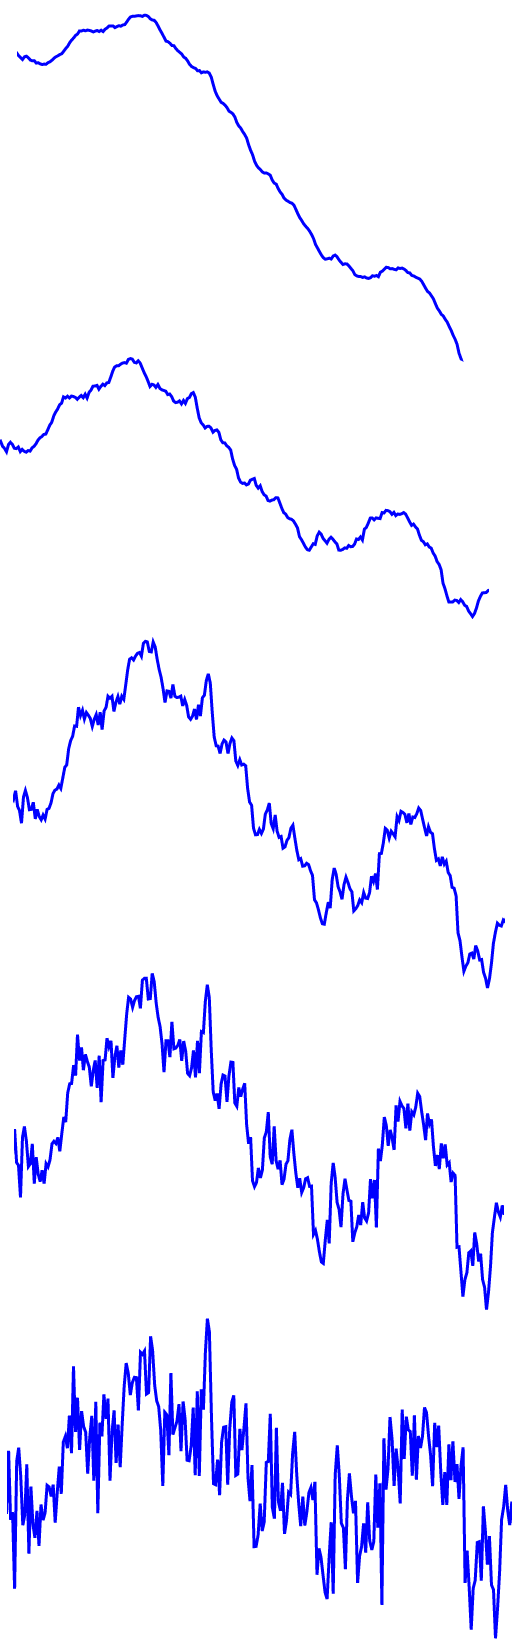
\includegraphics[width=11cm]{figures/hurst}
\caption{Curvas obtenida con distintos coeficientes de Hurst.}
\label{fg:hurst}
\end{figure}

Existen diversos métodos para computar el fBm en computación gráfica.
En \cite{Fournier1982} se presenta un método de subdivisión recursiva, denominado algoritmo de desplazamiento aleatorio del punto medio.

El algoritmo tiene su base en una fórmula de esperanza condicional para $B_{H}(u,w)$ \cite{Mandelbrot1968}, partiendo de $B_{H}(0,w) = 0$ y $B_{H}(1,w) = 1$, $0 \le u \le 1$ entonces $E[B_{H}(u,w)|B_{H}(1,w)] = \frac{1}{2} (u^{2H} + 1 - |u-1|^{2H})$.
Si $u=\frac{1}{2}$, entonces la esperanza es igual a $\frac{1}{2}$, independientemente de $H$.
Esto, junto al hecho de que el proceso es autosimilar, permite diseñar un algoritmo que subdivide el segmento en su punto medio, y al valor esperado para el punto medio se lo desplaza por un número aleatorio con media $0$ y variancia $1$ multiplicado por la variancia, la cual es igual a $2^{-H}$ ($2^{-H} * gauss(0,1) $).
Una vez computado el punto medio, el intervalo se subdivide y se computan de manera recursiva las mitades resultantes, donde la nueva variancia será proporcional al tamaño del nuevo segmento.

En la Fig.~\ref{fg:puntomedio} puede observarse un ejemplo de una curva obtenida utilizando distintas profundidades en el algoritmo recursivo.
Se observa que se puede obtener mayor detalle a mayor número de iteraciones, donde la curva resultante asemeja visualmente al perfil de una montaña.

\begin{figure}
\center
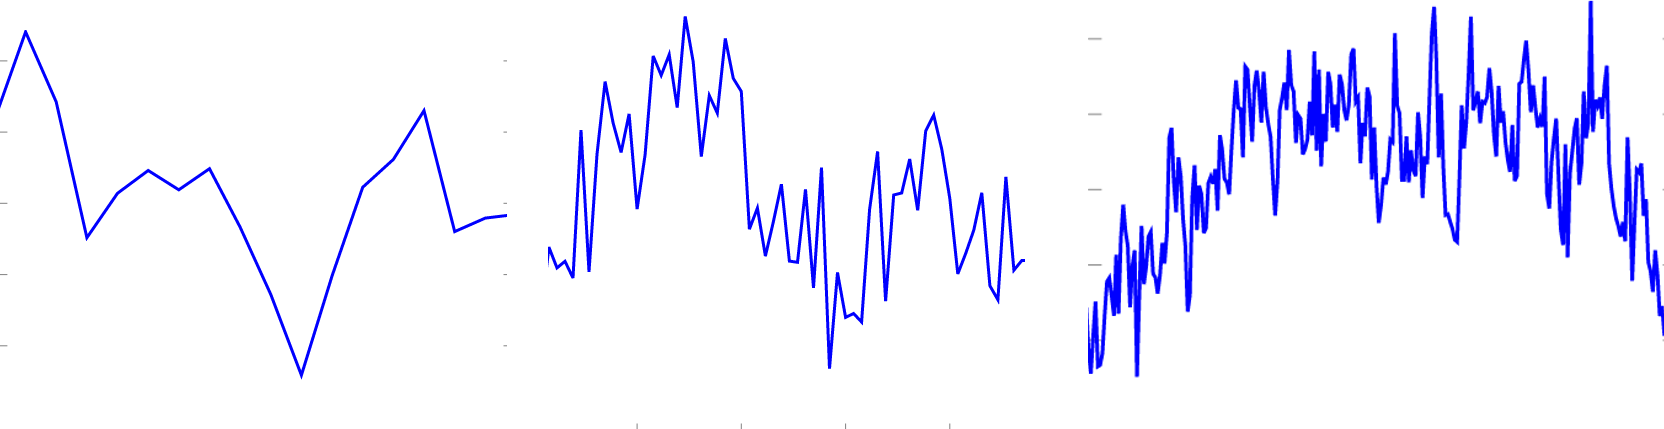
\includegraphics[width=11cm]{figures/puntomedio}
\caption{Curva obtenida con $H=0.8$, para $17$, $65$ y $257$ muestras, utilizando el algoritmo del punto medio.}
\label{fg:puntomedio}
\end{figure}


Una extensión directa de este algoritmo se da en dos dimensiones, donde los valores que se subdividen representan las alturas de un terreno.
Comenzando con $4$ puntos en un plano, formando un cuadrado, donde cada punto almacena la altura del terreno, es posible sudividir el terreno en $4$ cuadrados, a partir de los puntos medios de cada arista del cuadrado original.
Con $H$ es posible controlar la rugosidad del terreno.
La Fig.~\ref{fg:terreno} muestra un ejemplo de la renderización de un terreno generado utilizando este método, donde $H = 0.9$, en la Fig.~\ref{fg:terreno2} $H = 0.3$.
Se puede observar que a medida que $H$ es mayor, el terreno es más suave.

\begin{figure}
\center
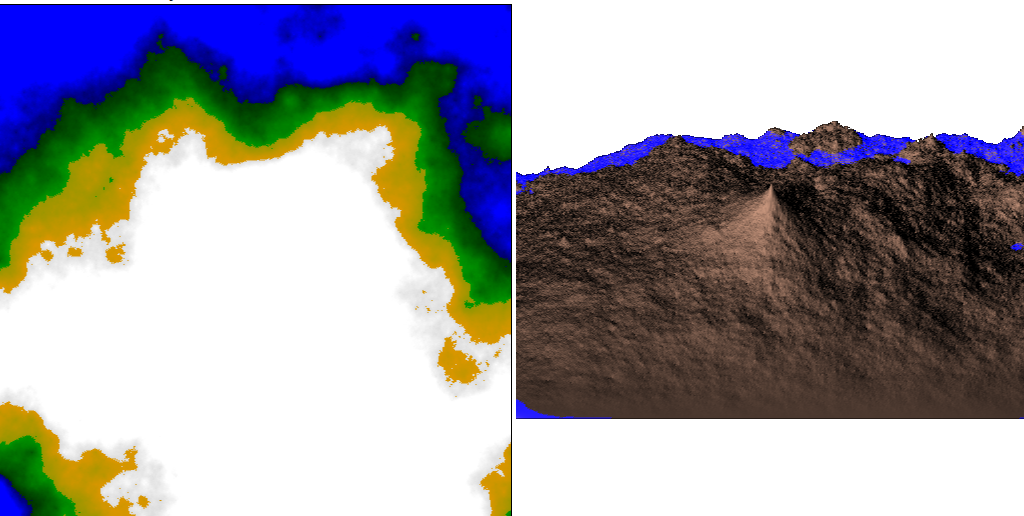
\includegraphics[width=11cm]{figures/terreno}
\caption{Terreno generado utilizando el algoritmo de desplazamiento del punto medio en dos dimensiones, con $H = 0.9$. La imagen de la izquierda muestra colores agregados de acuerdo al número generado, la imagen de la derecha muestra un ejemplo tridimensional de los mismos datos visto en perspectiva.}
\label{fg:terreno}
\end{figure}

\begin{figure}
\center
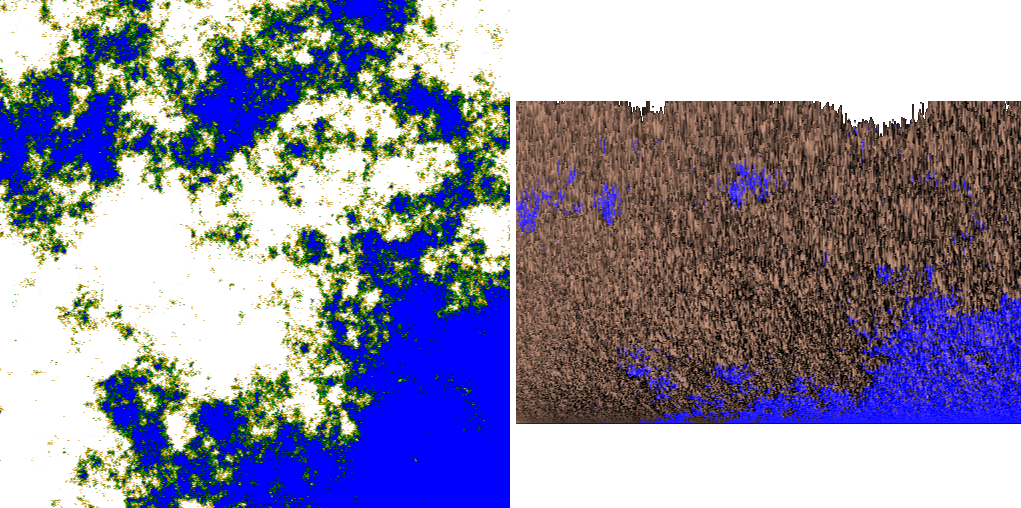
\includegraphics[width=11cm]{figures/terreno2}
\caption{Terreno generado utilizando el algoritmo de desplazamiento del punto medio en dos dimensiones, con $H = 0.3$.}
\label{fg:terreno2}
\end{figure}

%\subsubsection{Planetas}
%\cite{Ebert2002}


\subsection{Modelos Físicos}
Si bien los resultados obtenidos por los modelos presentados hasta ahora son muy satisfactorios, existe aún la necesidad de no depender de parámetros ad-hoc, además de aumentar el realismo de las imágenes resultantes.
Hasta aquí, la utilización de los modelos se basa casi exclusivamente en su {\em parecido visual} a los objetos que se intentan modelar.

Para poder mejorar esto es necesario utilizar los procesos físicos de formación o comportamiento de los materiales (movimiento de partículas, deformaciones, cambios químicos, etc.), lo cual permitiría definir parámetros más intuitivos que tienen su correlación en la realidad, logrando además una representación más exacta de la misma.
La desventaja de utilizar modelos físicos o matemáticos, recae sobre los tiempos de cómputo y la dificultad de diseño de éstos.

Sin embargo, desde el surgimiento del área, estos modelos han ido evolucionando gracias al incremento en el poder de cómputo del hardware gráfico disponible. A pesar de esto, aún nos encontramos en los comienzos de la utilización masiva de los mismos, por lo cual existen sólo unos pocos casos en los que se utilizan modelos de primeros principios.
En esta sección presentamos un ejemplo de esto, lo cual ejemplifica la capacidad de representación que puede alcanzarse al agregar detalles reales en las implementaciones.

\subsection{Fluídos}
Entre los primeros intentos por utilizar procesos físicos para modelar la apariencia de los materiales, encontramos ecuaciones que describen fluidos.
Las ecuaciones de Navier-Stokes describen un fluído cuya temperatura es prácticamente constante por medio de un campo de velocidades $\bold{u}$ y un campo de presiones $p$.
Dadas condiciones iniciales para $\bold{u}$ y $p$ cuando $t = 0$, la evolución de las cantidades puede describirse como sigue, independientemente del número de dimensiones,

\begin{align}
\nabla \cdot \bold{u} &= 0, \label{eq:eq1}\\
\frac{\partial \bold{u} }{\partial t} &= - (\bold{u} \cdot \nabla) \bold{u} - \frac{1}{\rho} \nabla p + \nu \nabla^{2} \bold{u} + \bold{f} \label{eq:eq2},
\end{align}

donde $\nu$ es la viscosidad cinemática del fluído, $\rho$ es la densidad y $\bold{f}$ es una fuerza externa.
Las ecuaciones modelan la conservación de masa (\ref{eq:eq1}) y de momento (\ref{eq:eq2}).

Además, deben tenerse en cuenta condiciones de borde.
Las mismas pueden variar en complejidad.
Por ejemplo, una implementación sencilla puede darse utilizando condiciones de borde periódicas, es decir, sin la existencia de {\em paredes} (el fluido se repite indefinidamente, este es el caso utilizado en el trabajo descripto aquí).
Un caso más complicado es una condición diferencial que describe el intercambio de masa con el ambiente.

Es posible combinar ambas ecuaciones para obtener una única ecuación de la velocidad.
Para esto, utilizaremos la descomposición Helmholtz-Hodge \cite{Chorin1990}, la cual establece que un campo vectorial $\bold{w}$ puede descomponerse como sigue, 

\begin{equation}
\label{eq:eq3}
\bold{w} = \bold{u} + \nabla q,
\end{equation}

donde $\bold{u}$ tiene divergencia $0$, es decir $\nabla\cdot\bold{u} = 0$.
Entonces, podemos definir un operador $\bold{P}$, el cual proyecta un campo vectorial $\bold{w}$ en su parte de divergencia $0$, $\bold{u} = \bold{P}\bold{w}$.
Dicho operador se puede definir implícitamente multiplicando $\nabla$ en ambos términos en la ecuación (\ref{eq:eq3}),

\begin{equation}
\label{eq:eq4}
\nabla\cdot\bold{w} = \nabla^{2} q.
\end{equation}

Una solución a esta ecuación está dada por

\begin{equation}
\label{eq:eq5}
\bold{u} = \bold{P}\bold{w} = \bold{w} - \nabla q,
\end{equation}

Si aplicamos el operador $\bold{P}$ en ambos lados de la ecuación (\ref{eq:eq2}), obtenemos una ecuación única para la velocidad,

\begin{equation}
\frac{\partial \bold{u} }{\partial t} = \bold{P} (- (\bold{u} \cdot \nabla) \bold{u} + \nu \nabla^{2} \bold{u} + \bold{f}) \label{eq:eq6},
\end{equation}

ya que $\bold{P}\bold{u} = \bold{u}$ y $\bold{P}\nabla p = 0$.
Esta ecuación es utilizada para derivar un algoritmo práctico para implementar apariencia de fluídos \cite{Stam1999}.
En la ecuación pueden verse un paso difusivo $\nu \nabla^{2} \bold{u}$, un paso de advección $- (\bold{u} \cdot \nabla) \bold{u}$ y una fuerza final aplicada $\bold{f}$.
Estos términos pueden resolverse por medio de la aplicación de métodos numéricos clásicos (por ejemplo diferencias finitas), por lo cual la solución final consiste en aplicar sucesivamente cada paso para obtener soluciones al campo vectorial $u$ en cada instante de tiempo $t$, finalmente proyectando el resultado con $P$.
El paso más complicado es el paso de proyección $P$, el cual se resuelve por medio de sistemas lineales, teniendo en cuenta que es un proceso de Poisson.

Cuando se conocen las velocidades $\bold{u}$, es posible aplicarlas a la utilización de partículas sobre el fluido, para proceder luego a su renderizado.

Este método se utiliza para modelar el comportamiento de agua y otros líquidos, además de algunos gases, nubes y humo, ver Figs.~\ref{fg:fluidos1},\ref{fg:fluidos2}.
La utilización de los procesos físicos subyacentes produce mayor realismo en el resultado que utilizar métodos heurísticos.
Desafortunadamente muchas veces esto resulta prohibitivo, no solo por costos computacionales, sino también por la complejidad en el diseño de los métodos, ya que se requiere muchas veces la participación de personas idóneas en la física utilizada.


\begin{figure}
\center
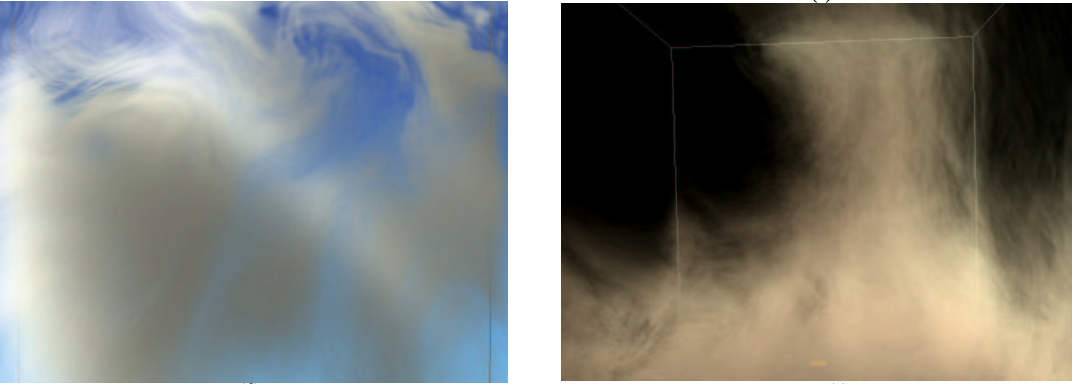
\includegraphics[width=11cm]{figures/fluidos1}
\caption{Nubes y humo generados utilizando métodos basados en las ecuaciones de Navier-Stokes.}
\label{fg:fluidos1}
\end{figure}

\begin{figure}
\center
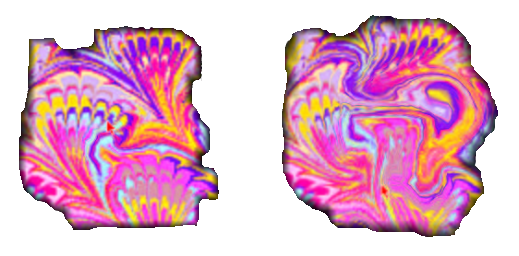
\includegraphics[width=11cm]{figures/fluidos2}
\caption{Fluidos generados utilizando métodos basados en las ecuaciones de Navier-Stokes.}
\label{fg:fluidos2}
\end{figure}

%\subsubsection{Telas}

\section{Representación Visual (Renderizado)}

Los materiales, además de presentar una geometría compleja, también presentan fenómenos particulares de interacción con la luz, los cuales incluyen translucencia, reflectancia, absorción, etc.
Debido a esto, en la década de $1980$ se simplificaron determinadas ecuaciones físicas para ser implementadas en computación gráfica, permitiendo modelar la apariencia de una gran variedad de materiales.

\subsection{Ecuación del Renderizado}

Esta ecuación modela el comportamiento de la luz en distintos tipos de superficie,

\begin{equation}
I(x,x') =  g(x,x')  \left[ \epsilon(x,x') + \int_{s}{\rho(x,x',x'')I(x,x'') dx''} \right],
\end{equation}
donde $I(x,x')$ es la intensidad de la luz que viaja de $x'$ a $x$ (sin oclusiones), $g(x,x')$ es un termino geométrico que modela la oclusión que podría existir entre $x$ y $x'$, $\epsilon(x,x')$ es la intensidad de la luz emitida desde $x'$ a $x$, $\rho(x,x',x'')$ es la intensidad de la luz emitida de $x''$ a $x$ por medio de una superficie en $x'$ (esta cantidad será llamada BRDF en una sección posterior), y $S=\bigcup{s_{i}}$ es la unión de todas las superficies de la escena.
De esta forma, $x$,$x'$ y $x''$ varían sobre todas las superficies de la escena.
La ecuación es una aproximación a la ecuación del electromagnetismo de Maxwell, pero sólo tiene en cuenta fenómenos óptico-geométricos.
Además se asume una superficie $S_{0}$, la cual es un semi-hemisferio que engloba a toda la escena.
$I(x,x')$ significa la radiación de energía por unidad de tiempo por unidad de superficie de destino por unidad de superficie de origen ($joule/m^{4} s$).
El término geométrico se hace $0$ si los puntos en consideración no son mutuamente visibles.

Por medio del modelado de cada término de forma separada, es posible obtener una gran cantidad de superficies.
Trabajos previos a la aparición de la ecuación del renderizado habían logrado resultados parciales, sin saber que una única ecuación podía englobar todos los fenómenos en investigación hasta ese entonces.
Como resultado de este modelo, hoy es posible llamar a los métodos previos a este como especializaciones o casos particulares de la ecuación del renderizado.

Fuera de la ecuación quedan efectos más complejos, como la difracción y la polarización.
De esta forma, la ecuación modela el comportamiento de la luz entre las superficies de la escena.
Más detalles de la misma pueden ser consultados en \cite{Kajiya1986}.

Si lo que se pretende modelar son fenómenos volumétricos, entonces debe atenderse a ciertas generalizaciones de la ecuación, como se ve en la siguiente sub-sección.

\subsection{Ecuación del Renderizado de Volúmenes}

Cuando un fotón de un rayo de luz atraviesa un medio en una dirección dada, pueden ocurrir dos eventos: el fotón es absorbido, o bien es redirigido en otra dirección, esto depende del coeficiente de absorción del medio $\sigma_{a}$ y el coeficiente de dispersión $\sigma{s}$.
La suma de ambos resulta en el coeficiente de extinción $\sigma_{t}$.

Si se escribe el coeficiente de absorción como $\sigma_{a}(\bold{x} + t\vec{\omega})$ , entonces una fracción de fotones absorbidas en un segmento de recta es notada como $\sigma_{a}(\bold{x} + t\vec{\omega}) \Delta t$.
Consecuentemente la fracción de fotones que escapa a la absorción en ese segmento de recta resulta,

$$L((\bold{x}+t\vec{\omega}) \rightarrow \vec{\omega}) = L(\bold{x} \rightarrow \vec{\omega}) (1-\sigma_{a}(\bold{x} + t\vec{\omega}) \Delta t),$$

o, de otra forma:

$$\frac{L((\bold{x}+t\vec{\omega}) \rightarrow \vec{\omega}) - L(\bold{x} \rightarrow \vec{\omega}) }{ \Delta t } = - L(\bold{x} \rightarrow \vec{\omega}) \sigma_{a}(\bold{x} + t\vec{\omega}).$$

Tomando el límite cuando $\Delta t \rightarrow 0$ se obtiene la derivada, es decir, el cambio diferencial en radiancia dado por la absorción del medio,

$$\lim_{\Delta t \rightarrow 0} \frac{L((\bold{x}+t\vec{\omega}) \rightarrow \vec{\omega}) - L(\bold{x} \rightarrow \vec{\omega}) }{ \Delta t } = - \sigma_{a}(\bold{x}) L(\bold{x} \rightarrow \vec{\omega})  = -(\vec{\omega} \cdot \nabla_{a}) L(\bold{x} \rightarrow \vec{\omega}),$$

donde $\nabla_{a}$ denota el gradiente dado por la absorción y $ \vec{\omega} \cdot \nabla_{a}$ expresa la derivada direccional de la absorción del medio en dirección $\vec{\omega}$.

Similarmente se halla el cambio en radiancia debido a la dispersión saliente,

$$ (\vec{\omega} \cdot \nabla_{o}) L(\bold{x} \rightarrow \vec{\omega}) = -\sigma_{s}(\bold{x}) L(\bold{x} \rightarrow \vec{\omega}),$$

de esta forma se pueden aunar ambos términos para expresar el cambio en radiancia debido a la extinción,

$$(\vec{\omega} \cdot \nabla_{t}) L(\bold{x} \rightarrow \vec{\omega}) = -(\sigma_{a}(\bold{x})+\sigma_{s}(\bold{x})) L(\bold{x} \rightarrow \vec{\omega}) = -\sigma_{t}(\bold{x}) L(\bold{x} \rightarrow \vec{\omega}).$$

Gracias a la expresión de arriba se puede calcular una cantidad de interés, llamada {\em Transmitancia}, $T_{r}$, la cual describe la cantidad de fotones que pueden viajar sin obstrucciones entre dos puntos en un medio (es decir en línea recta).
Integrando la ecuación anterior se obtiene,

$$T_{r}(\bold{x'} \leftrightarrow \bold{x}) = e^{-\tau(\bold{x'} \leftrightarrow \bold{x})},$$

donde $\tau$ recibe el nombre de densidad óptica del material y su expresión es,

$$\tau(\bold{x'} \leftrightarrow \bold{x}) = \int_{0}^{d} -\sigma_{t}(\bold{x}+t\vec{\omega})dt$$,

con $t \in [0,d]$.
La ecuación es el resultado de integrar la extinción a lo largo del segmento de recta.


Hasta ahora se describió la pérdida de fotones a medida que un rayo de luz viaja por un medio.
Similarmente existen dos fenómenos que provocan que fotones que previamente no estaban presentes en el rayo de luz se sumen al mismo.
El primero es llamado dispersión entrante, y consiste en el rebote de fotones que provocan que los mismos adopten la dirección del rayo actual.
Su expresión matemática es

$$ (\vec{\omega} \cdot \nabla_{i}) L(\bold{x} \rightarrow \vec{\omega}) = \sigma_{s}(\bold{x}) L_{i}(\bold{x} \rightarrow \vec{\omega}).$$

El último fenómeno aparece en medios que transforman otras formas de energía como el calor, en luz visible, y se llama emisión, con expresión

$$ (\vec{\omega} \cdot \nabla_{e}) L(\bold{x} \rightarrow \vec{\omega}) = \sigma_{a}(\bold{x}) L_{e}(\bold{x} \rightarrow \vec{\omega}).$$

La ecuación en su forma completa representa el comportamiento de la luz en volúmenes, considerando los cuatro fenómenos

\begin{equation}
\begin{aligned}
(\vec{\omega} \cdot \nabla) L(\bold{x} \rightarrow \vec{\omega}) = - \sigma_{a}(\bold{x}) L(\bold{x} \rightarrow \vec{\omega}) - \sigma_{s}(\bold{x}) L(\bold{x} \rightarrow \vec{\omega}) + \\
\sigma_{a}(\bold{x}) L_{e}(\bold{x} \rightarrow \vec{\omega}) + \sigma_{s}(\bold{x}) L_{i}(\bold{x} \rightarrow \vec{\omega}).
\end{aligned}
\end{equation}

La misma expresa que el cambio ($\nabla$) de radiancia $L$ de un rayo de luz a lo largo de un medio, en una dirección dada ($\vec{\omega}$) está dado por cuatro fenómenos:   absorción, dispersión saliente, emisión (del medio) y dispersión entrante, ver Fig.~\ref{fg:fenomenosrte}.
Esta ecuación recibe el nombre de ecuación de transporte radiativo (Radiative Transport Equation, RTE) \cite{Chandrasekhar1960}.

Podemos expresar esta ecuación en forma integral integrando ambos lados de la igualdad, y asumiendo como condición de borde a la ecuación del renderizado de la sección anterior, obteniendo,

\begin{equation}
\begin{aligned}
L(\bold{x} \leftarrow \vec{\omega}) = T_{r}(\bold{x} \leftrightarrow \bold{x_{s}}) L(\bold{x_{s}} \rightarrow -\vec{\omega}) + \\
\int_{0}^{s}{T_{r}(\bold{x} \leftrightarrow \bold{x_{t}}) \sigma_{a}(\bold{x}) L_{e}(x \rightarrow -\vec{\omega}) dt } + \\
\int_{0}^{s}{T_{r}(\bold{x} \leftrightarrow \bold{x_{t}}) \sigma_{a}(\bold{x_{t}}) L_{i}(x_{t} \rightarrow -\vec{\omega})  }
\end{aligned}
\end{equation}

donde $L(\bold{x} \leftarrow \vec{\omega})$ describe la radiancia que llega a $\bold{x}$ desde $\bold{\omega}$, $s$ es el ancho del medio desde $\bold{x}$ en dirección $\vec{\omega}$, $\bold{x_{t}} = \bold{x} + t\vec{\omega}$ con $t \in (0,s)$ y $\bold{x_{s}} = \bold{x}+ s\vec{\omega}$ es un punto en una superficie más allá del medio, ver Fig.~\ref{fg:rte}.
El primer término de la ecuación representa radiancia entrando por detrás del medio.
El segundo, la emisión de radiancia en el medio.
El último, la acumulación de radiancia entrante al medio. 

Esta ecuación es aún más compleja que la ecuación del renderizado presentada en la sección anterior.
Cada punto del medio depende de {\em todos} los demás puntos del medio, por lo que deben desarrollarse métodos que permitan computar aproximaciones adecuadas de la misma.
Simplificaciones usuales incluyen ignorar el término de emisión, y asumir un medio isotrópico u homogéneo.

Diversos algoritmos específicos surgieron con anterioridad a estas ecuaciones generales, y sin saberlo, formaban parte de un mismo marco teórico, las cuales hoy por hoy son algoritmos especializados para ciertos tipos de materiales y situaciones, entre ellos se encuentran el trazado de rayos \cite{}, la radiosidad \cite{} y el mapeo de fotones \cite{}.



\begin{figure}
\center
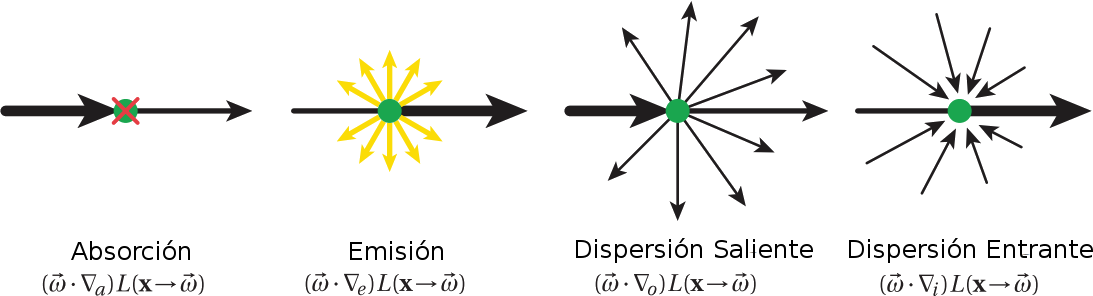
\includegraphics[width=11cm]{figures/fenomenosrte}
\caption{Fenómenos intervinientes en la Ecuación del Transporte Radiativo.}
\label{fg:fenomenosrte}
\end{figure}

\begin{figure}
\center
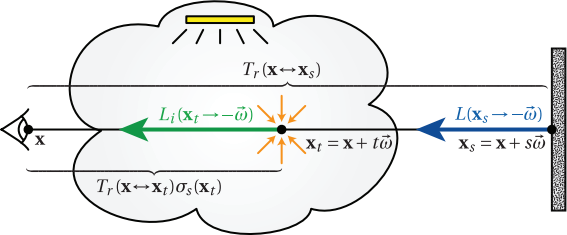
\includegraphics[width=11cm]{figures/rte}
\caption{Interpretación gráfica de la Ecuación del Transporte Radiativo.}
\label{fg:rte}
\end{figure}


%\section{Simplificaciones a las Ecuaciones de Renderizado}
\section{Funciones de Distribución de Reflectancia (BRDFs)}
\subsection{Motivación}
En la ecuación del renderizado se introdujo un término llamado BRDF, el cual es una función que modela el comportamiento de la luz en relación con una superficie determinada.
Diversos fenómenos tienen lugar cuando un rayo de luz impacta una superficie de un objeto.
En su máxima expresión, una BRDF podría tomar en consideración variables como la longitud de onda a ser representada, la posición de salida del rayo reflejado en la superficie, e incluso el tiempo de demora entre la entrada y la salida del rayo.
Gracias a esto, sería posible modelar fenómenos tan complejos como la fosforescencia y la polarización.
Como puede imaginarse, una complejidad como esta no resulta algo práctico a ser utilizado en computación gráfica, por lo cual deben realizarse simplificaciones sobre los materiales subyacentes.
Una simplificación muy común de esta función consiste en ignorar los fenómenos anteriores y limitar la definición de la BRDF a un par de ángulos de entrada y de salida, para cada punto de la superficie.
De cualquier manera, esta simplificación es todavía una función de $6$ variables, que incluye los cuatro números que definen el ángulo de entrada y de salida, y los dos que se corresponden a una representación paramétrica de una superficie.
Debido complejidad aún presente en la definición, los primeros modelos utilizados en computación gráfica eran funciones analíticas \cite{Phong1975,Blinn1977}, es decir, una función simple que no requería almacenamiento de datos (ya que el valor se calcula en el momento de llamar a la función).
De esta manera fue posible representar diversos materiales sencillos, sobre todo metales y objetos con una marcada reflectancia, aunque de una manera que no estaba basada en ningún procedimiento de obtención, sino más bien en un procedimiento artístico que producía resultados aceptables.
Posteriormente surgieron modelos más precisos, los cuales desarrollaron funciones analíticas más ajustadas al fenómeno real, el cual es comparado por medio de mediciones.
Es decir, se captura de manera más precisa la reflectancia de la superficie de determinados materiales \cite{He1991,Ward1992,Lafortune1997}.
Para esto, se modelaron las anisotropías propias de los materiales (cambio de reflectancia para distintos ángulos), o sea, la no linealidad de las BRDF, lo cual otorga un mayor realismo.
Además, otros trabajos \cite{Dana1999,Matusik2003} realizaron mediciones de la reflectancia de materiales por medio de dispositivos de captura (goniorreflectómetros), lo cual constituye una solución de fuerza bruta, pero adecuada en algunos casos.
Los datos de las mediciones del material generalmente son publicados para uso de la comunidad gráfica y científica.
Finalmente, es posible intentar representar los datos mesurados en materiales reales con modelos matemáticos, buscando reducir costos de almacenamiento \cite{Ngan2005}.

\subsection{Definición}
Previamente definimos la BRDF como una función matemática que tomaba como parámetro tres puntos del espacio.
Una forma equivalente consiste en definir, para cada punto de una superficie, el ángulo de entrada y salida del rayo

$$\rho(\theta_{i},\phi_{i},\theta_{r},\phi_{r}) = \frac{dL_{r}(\theta_{r},\phi_{r})}{dE_{i}(\theta_{i},\phi_{i})},$$

donde $E$ es la {\em irradiancia}, que se define como flujo incidente sobre unidad de área, y $L$ es la radiancia reflejada.
Intuitivamente, la BRDF mide la cantidad de luz reflejada a partir de la cantidad de energía incidente en la superficie, para cada ángulo de entrada y de salida.

Muchas BRDF modelan por separado determinadas características comunes en materiales.
Por ejemplo, las contribuciones especulares (reflejos perfectos) y difusa (la luz se disipa en todas las direcciones de manera equitativa).
La primera produce diferencias visibles en superficies, siendo característicos patrones blancos (como círculos, líneas) sobre determinadas direcciones de rebote.

La Fig.~\ref{fg:contribuciones} muestra ejemplos de estos rebotes.
Las direcciones de reflejo suelen formar patrones llamados lóbulos, los cuales permiten entender intuitivamente el comportamiento de la BRDF (a simple vista, es posible saber la dirección donde se dirigirán más rayos y por lo tanto, mayor radiancia).
Si el observador se coloca en la dirección de reflejo de estos lóbulos, verá mayor radiancia que en otras direcciones.

\begin{figure}
\center
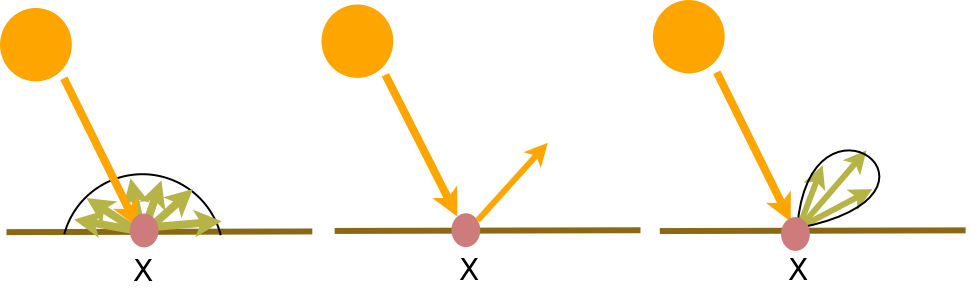
\includegraphics[width=11cm]{figures/contribuciones}
\caption{Diferentes comportamientos posibles de BRDFs. La imagen de la izquierda muestra una reflexión difusa, la del centro, una completamente especular, y la de la derecha, lobular.}
\label{fg:contribuciones}
\end{figure}

La Fig.~\ref{fg:microestructura} muestra un ejemplo de una geometría microscópica de un material y su BRDF resultante.
Como puede observarse, la apariencia final de la BRDF depende de la orientación de determinadas estructuras presentes a escalas microscópicas del material.
En algunos casos es posible asumir distribuciones estadísticas, pero en la mayoria de los materiales esto no es así.
La microgeometría es lo suficientemente compleja como para presentar anisotropías y formas de apariencia caprichosa.
Como fue dicho, si no es posible modelar matemáticamente el comportamiento del material, muchas veces se recurre a mediciones sobre muestras reales.


\begin{figure}
\center
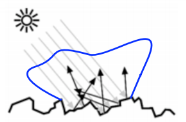
\includegraphics[width=5cm]{figures/microestructura}
\caption{Explicación del comportamiento observable en BRDFs.}
\label{fg:microestructura}
\end{figure}


\begin{figure}
\center
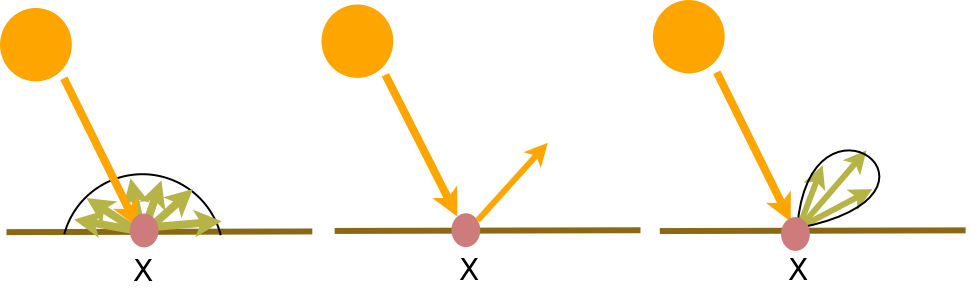
\includegraphics[width=11cm]{figures/contribuciones}
\caption{Diferentes comportamientos posibles de BRDFs. La imagen de la izquierda muestra una reflexión difusa, la del centro, una completamente especular, y la de la derecha, lobular.}
\label{fg:contribuciones}
\end{figure}


Un ejemplo muy común de BRDF es el modelo de Phong, ver Fig~\ref{fg:phongVecs}, el cual presenta la siguiente definición matemática:

$$\rho_{phong} =  k_{a} I_{a} + k_{d} max((N \cdot L),0) + k_{s} (R \cdot V)^{\alpha},$$

donde $k_{a}$, $k_{d}$ y $k_{s}$ son coeficientes de iluminación ambiente, difusa y especular, el vector $N$ es el normal a la superficie, $R$, el reflejado, $V$ el vector que va desde la superficie hacia la posición del observador y $L$ la fuente de luz, y $\alpha$ es un parámetro que determina el brillo final de los reflejos del material, ver Fig.~\ref{fg:phongparametros}.
Si bien el modelo es completamente fenomenológico, el mismo es flexible y obtiene buenos resultados para materiales simples.


\begin{figure}
\center
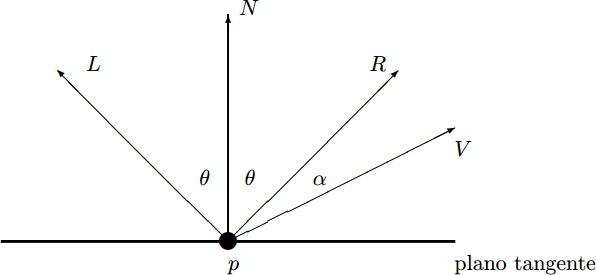
\includegraphics[width=11cm]{figures/phongVecs}
\caption{Vectores intervinientes en el cómputo de la BRDF de Phong.}
\label{fg:phongVecs}
\end{figure}

\begin{figure}
\center
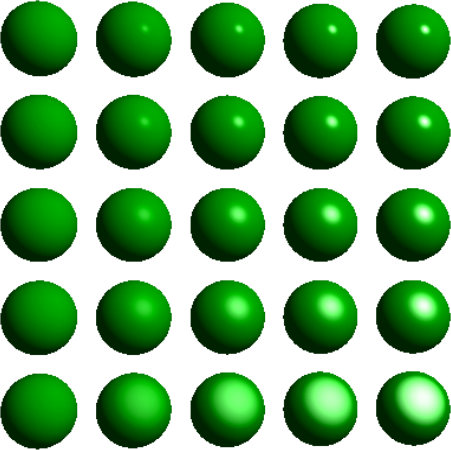
\includegraphics[width=9cm]{figures/phongparametros}
\caption{Diferentes Parámetros en el modelo de Phong. De izquierda a derecha $k_{s}$ varía de $0$ a $1$. De arriba hacia abajo, $\alpha$ varía de $50$ a $1$.}
\label{fg:phongparametros}
\end{figure}


%Un ejemplo simple de una BRDF es una superficie Lambertiana perfectamente difusa.
%La BRDF resulta constante

$$$$

%Todas estas simplificaciones son realizadas a escala humana, es decir, sin tener en consideración la naturaleza microscópica de la luz. En esta escala, las trayectorias que describe la luz son aproximadas por líneas rectas.
%\subsection{Radiosidad}


%\subsection{Ray Tracing}
%\subsection{Ray Marching}
%\subsection{Volume Rendering}
%\subsection{Photon Mapping}

\section{Materiales específicos}
Debido a la necesidad creciente de modelado realista de materiales, se desarrollaron técnicas específicas para materiales determinados, ya que los mismos no encajaban en el marco global de las técnicas desarrolladas a partir de las ecuaciones del renderizado.

Si bien las ecuaciones presentadas proveen un marco teórico general de los fenómenos que ocurren entre la luz y los materiales en una escena, los detalles de la implementación computacional muchas veces hace imposible una utilización directa de las mismas.

Debido a esto han surgido técnicas que buscando lograr un renderizado realista, han tenido que tener en cuenta el proceso de fabricación del material (por ejemplo en telas), o el diseño de las microgeometrías presentes en sus superficies (cerámicos).


Esta sección muestra claramente que el modelado y renderizado de materiales es un tema abierto, del cual sólo algunos ejemplos han sido desarrollados \cite{Dorsey2007}.
Existe aún un amplio abanico de materiales que no han sido modelados, y dependiendo del nivel de realismo deseado es posible aplicar diversas metodologías al diseño de los mismos.


\subsection{Piel}
Comenzaremos con un material extremadamente complejo y necesario en computación gráfica, la piel humana.
Existen para este material un importante número de trabajos científicos, presentando diversos enfoques a la hora de realizar su modelado.
Un modelo poco preciso de la piel puede ser fácilmente detectado por humanos, por lo cual un diseño cuidado es necesario para alcanzar un realismo aceptable.


La piel está fuertemente estudiada en medicina.
Debido a esto, existen trabajos muy completos sobre su estructura y propiedades \cite{Walters2002}.
La piel está compuesta por diversas capas como la epidermis, la dermis y la hipodermis.
La más exterior es la epidermis, compuesta por células muertas.
La siguiente capa en profundidad es la dermis, la cual es más ancha y posee vasos sanguíneos (lo cual afecta el color final de la piel).
La hipodermis es la capa más interna y conecta la piel con el cuerpo.
Todas estas capas presentan una estructura muy compleja.
Este material es muy dinámico, y puede ser afectado por diversos factores, como el sol, lastimaduras, y cambios en el torrente sanguíneo.
Su estructura geométrica también es compleja, presentando poros y por ejemplo, patrones característicos (por ejemplo las huellas digitales).

La estructura de capas fue imitada en computación gráfica, realizando simplificaciones.
De esta forma, se diseñó un modelo de reflectancia para su superficie (BRDF) y un modelo de dispersión debajo de la superficie (BSSRDF) en una segunda capa, junto con un modelo microgeométrico de la superficie.

Un ejemplo es \cite{Marschner2000}, el cual utiliza una BRDF de Lafortune (ver secciones anteriores) para la reflectancia superficial, junto con texturas que se mapean sobre una geometría de la cara de una persona.
En otro trabajo se agregó información proveniente de moldes de polímeros presionados sobre la cara de personas \cite{Haro2001}, con el fin de capturar detalles finos de la geometría, utilizando además algoritmos de síntesis de imágenes para generar muestras más grandes que las medidas, ver Fig.~\ref{fg:piel}.

\begin{figure}
\center
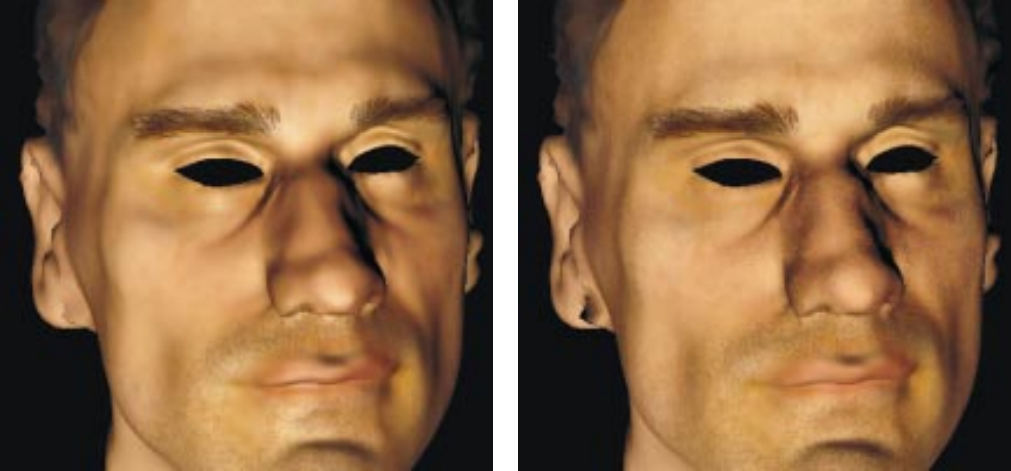
\includegraphics[width=9cm]{figures/piel}
\caption{Piel Humana renderizada con el método de \cite{Marschner2000}. La imagen de la derecha muestra la mejora obtenida al agregar detalles de geometría fina en el modelo (nariz, parte inferior del labio).}
\label{fg:piel}
\end{figure}

Un modelo basado en primeros principios puede verse en \cite{Krishnaswamy2004}.
En ese trabajo se definen geometrías precisas para la dermis y epidermis, a partir de la cual se realizan simulaciones físicas de rebote de la luz (simulaciones Monte Carlo), gracias a las cuales es posible reconstruir una BRDF.
El modelo incluye muchos otros detalles de los procesos físicos intervinientes, como la melanina, bilirrubina, absorción, pigmentación, etc.

Existen trabajos que abordan otros aspectos del modelado de la apariencia de la piel.
El estudio de los patrones que produce el envejecimiento es sujeto de estudio en \cite{Boissieux2000}.
Los mismos fueron medidos en muestras reales de una empresa cosmética.
También es posible obtener información geométrica fina a partir de imágenes \cite{Golovinskiy2006}.

\subsection{Materiales Porosos}
La utilización de superficies puede ser una limitación a la hora de modelar un material.
En el caso de los materiales porosos, existen micro-poros en la geometría, los cuales interaccionan con la luz, que hacen que los enfoques clásicos no sean adecuados.
Los poros mencionados son más pequeños que los poros de la piel humana.
Si bien son más grandes que la longitud de onda de la luz, los mismos no son visibles al ojo humano.

Entre los pocos trabajos sobre estos materiales, se encuentra \cite{Merillou2000}.
En dicho trabajo la BRDF estándar es modificada para incluir comportamiento de materiales porosos.
Para esto, se realizan simulaciones Monte Carlo sobre posibles configuraciones microscópicas de poros bajo ciertas asunciones.
Un ejemplo típico de poro puede verse en la Fig.~\ref{fg:poro}.
Se simula el rebote de la luz en la geometría sintetizada, y luego se computan las distribuciones para múltiples poros con distintas formas.
Con esto se modifican los coeficientes de especularidad y difusividad de la BRDF.
En la Fig.~\ref{fg:ceramico} podemos observar una imagen de una maceta renderizada con una BRDF tradicional, y a la derecha, la misma imagen utilizando este método.

\begin{figure}
\center
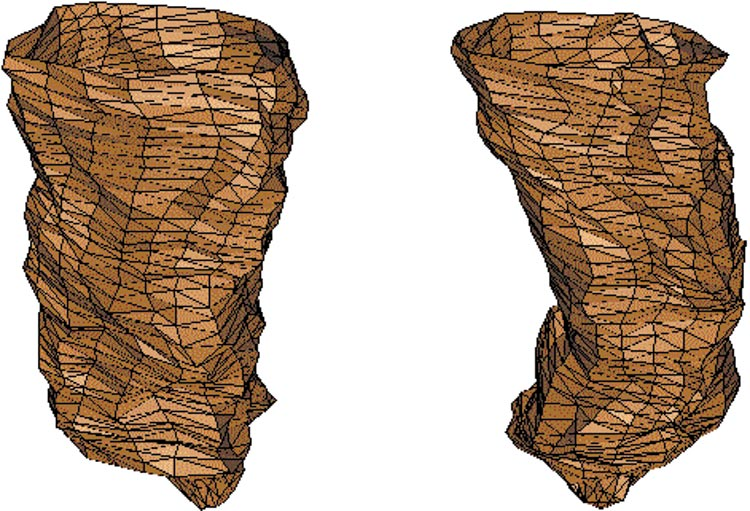
\includegraphics[width=8cm]{figures/poro}
\caption{Ejemplo de poros sintetizados utilizando el método de \cite{Merillou2000}.}
\label{fg:poro}
\end{figure}

\begin{figure}
\center
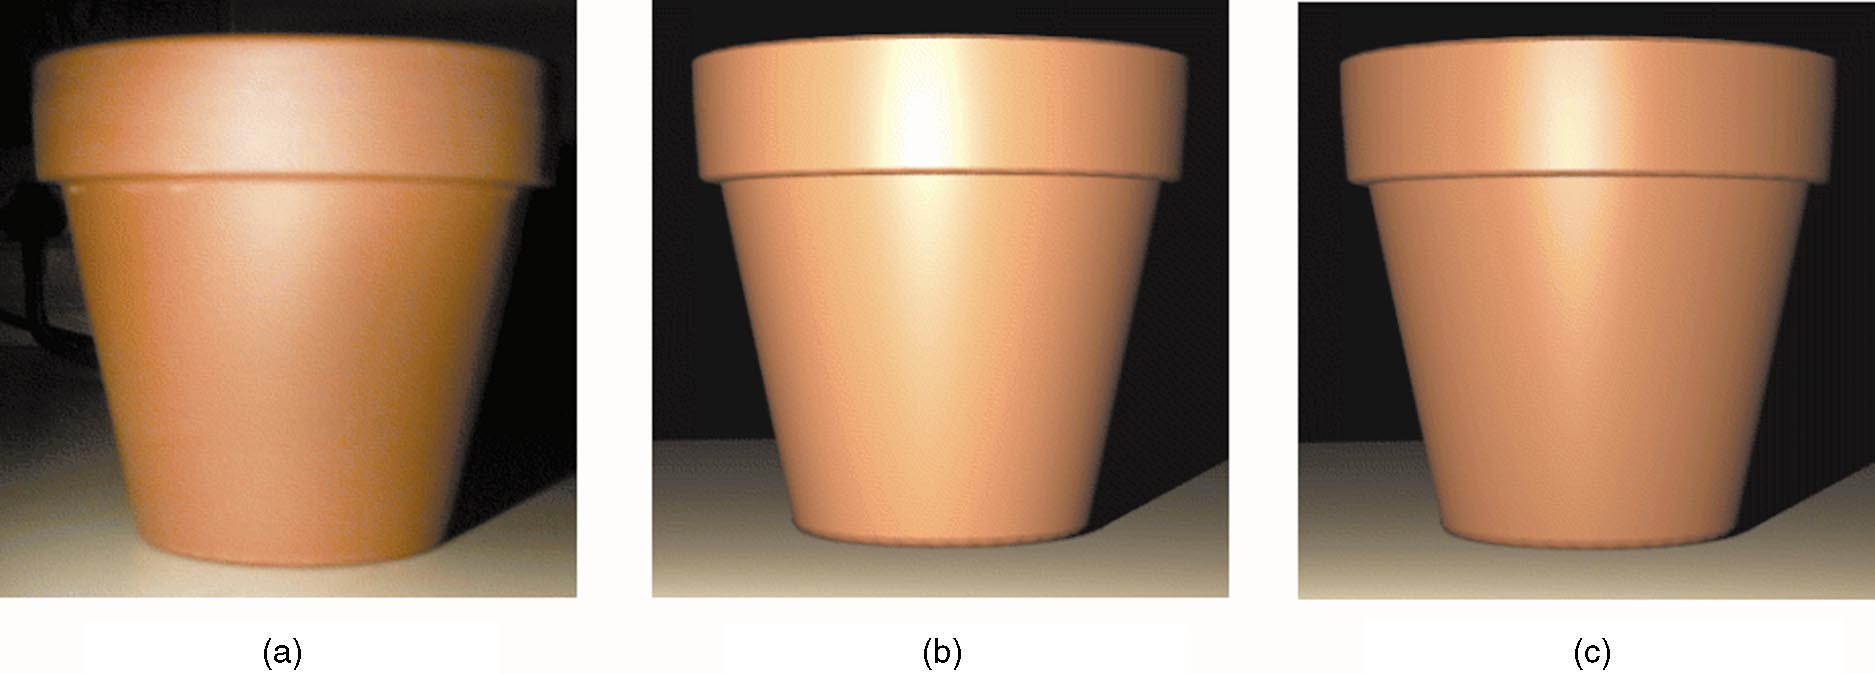
\includegraphics[width=11cm]{figures/ceramico}
\caption{Cerámicos renderizados. Izquierda: maceta real. Centro: utilizando una BRDF tradicional. Derecha: utilizando el método propuesto en \cite{Merillou2000}.}
\label{fg:ceramico}
\end{figure}

La tesis presente se ubica sobre este tipo de materiales.

\subsection{Pelo}
El mismo consiste de tres partes principales: una médula central, el córtex y una cutícula exterior.
Su color está dado por gránulos de melanina en el córtex.
Cuando no están presentes estos gránulos se observa un color blanco.


Existen dos tipos principales de pelo, uno es el vello, el cual crece en prácticamente todo el cuerpo, con $1$ {\em mm} de alto, y otro es el pelo terminal, el cual se encuentra en el cuero cabelludo.
Este último fue el que recibió mayor atención en computación gráfica.
El pelo terminal tiene aproximadamente entre $50$ y $90$ micrones de diámetro.
Existen entre $175$ y $300$ pelos terminales por {\em $cm^{2}$}.
El pelo de animales difiere del humano en color tamaño, y densidad.

Cada pelo individual puede considerarse una superficie con dispersión lumínica propia.
Por otro lado, la apariencia típica del pelo está dada por el conjunto de muchos pelos individuales.
Sin embargo, utilizar soluciones volumétricas típicas, como modelar el pelo como una nube o una nube no resulta adecuado, ya que la geometría del pelo afecta la reflectancia de la luz incidente.
Para solucionar estos inconvenientes se utilizar una estructura denominada {\em texel}, que no debe confundirse con un elemento de una textura.
Un texel es una {\em estructura de datos} volumétrica que asocia tres componentes: una densidad de área proyectada $\rho$, un marco de referencia $\bold{B}$ y un modelo bidireccional de reflexión de la luz $\psi$, a cada posición $3D$ del espacio.
La densidad de área proyectada $\rho$ es la fracción del área proyectada del voxel en una dirección particular que es cubierta por geometría del pelo proyectada en la misma dirección.
En $\bold{B}$, la orientación queda especificada por los vectores normal, binormal, y tangente.
Para determinar los vectores, se asume un cilindro general que crece desde la piel del cuero cabelludo.
$\psi$ se define como una variación del modelo de Phong, devolviendo la luz reflejada en el punto.
Los componentes difuso y especular del modelo son,

\begin{align*}
\psi_{d} &= K_{d} sin \theta_{i}\\
\psi_{s} &= K_{s} (cos \theta_{i} cos \theta_{r} + sin \theta_{i} sin \theta_{r})^{p},
\end{align*}

donde $\theta_{i}$ es el ángulo entre la luz y la tangente al pelo, y $\theta_{r}$ es el ángulo entre la tangente al pelo y el observador.

Luego, para calcular el color final de un pixel visto desde el observador en pantalla, se recorren en línea recta, desde $t_{near}$ a $t_{far}$ según corresponda a ese pixel, los texels necesarios,

$$L = \sum_{t=t_{near}}^{t=t_{far}} {e^{-\tau \sum_{u=t_{near}}^{u=t} \rho(u)} \rho(t) \sum_{i} L_{i}(t) \bold{\psi}(t)},$$

donde la suma sobre $i$ refiere a las fuentes de luz, y $\tau$ es un coeficiente que convierte las distribuciones de área proyectada en un coeficiente de atenuación.

Este método sirve para simular pelo corto, pero visto a cierta distancia, ver Fig.~\ref{fg:osopelo}.
La percepción de pelo se pierde cuando la cámara se acerca demasiado al objeto.

\begin{figure}
\center
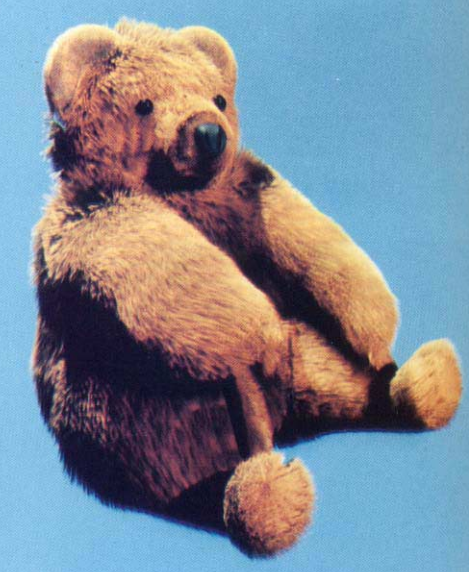
\includegraphics[width=6cm]{figures/osopelo}
\caption{Ejemplo de renderizado de pelo en un oso de peluche con el método propuesto en \cite{Kajiya1989}.}
\label{fg:osopelo}
\end{figure}

%The projected area density is the fraction of the projected area of the voxel in a particular direction that is covered by hair geoemetry projected in the same direction

Es posible mejorar el método por medio de otras funciones $\bold{\psi}$, teniendo en cuenta factores como la transmitancia y el impacto de las fibras individuales entre sí (iluminación indirecta).
Puede verse un estudio más completo de la literatura sobre renderizado de pelo en \cite{Ward2007}.

\subsection{Telas}
Las telas son un material similar al pelo en el sentido de que su apariencia está basada en un conjunto de fibras.
Las fibras de telas presentan diferentes {\em tinturas}.
Es importante tener en cuenta las tinturas para entender la apariencia de una tela cuando es vista desde distintos ángulos.
Por ejemplo, determinadas fibras de telas presentan más de una tintura, como muestra la Fig.~\ref{fg:fibra}.
En este caso, los rayos de luz que llegan desde distintas posiciones atraviesan distintas longitudes sobre las tinturas, produciendo iridiscencia, es decir, cambio de color visible dependiendo del ángulo de visión.

\begin{figure}
\center

\includegraphics[width=4cm]{figures/fibra}
\caption{Ejemplo de fibra de tela con más de una tintura. Se puede observar una tintura roja en el centro, y una tintura azul que la envuelve.}
\label{fg:fibra}
\end{figure}

La apariencia de cada tipo de tela es diferente, y depende del material utilizado (seda, lana, hilos, etc.) como del proceso de tejido en sí.
En \cite{Xu2001} se observa que determinados hilos están formados por un conjunto de fibras, apretados y con estructura helicoidal.
Esta observación se aprovecha para definir un texel específico como en el caso del pelo, el cual luego permite determinar la cantidad de luz que será emitida en una dirección para una dirección entrante.
Para esto se tienen en cuenta efectos como sombras, oclusión y dispersión múltiple entre los distintos hilos que componen una tela.
Debe contarse además con una estructura coherente que conecte a los hilos, formando una tela realista.
Para esto se utilizan curvas $3D$ construídas a partir de los puntos de control definidos en la división de la superficie.


\begin{figure}
\center
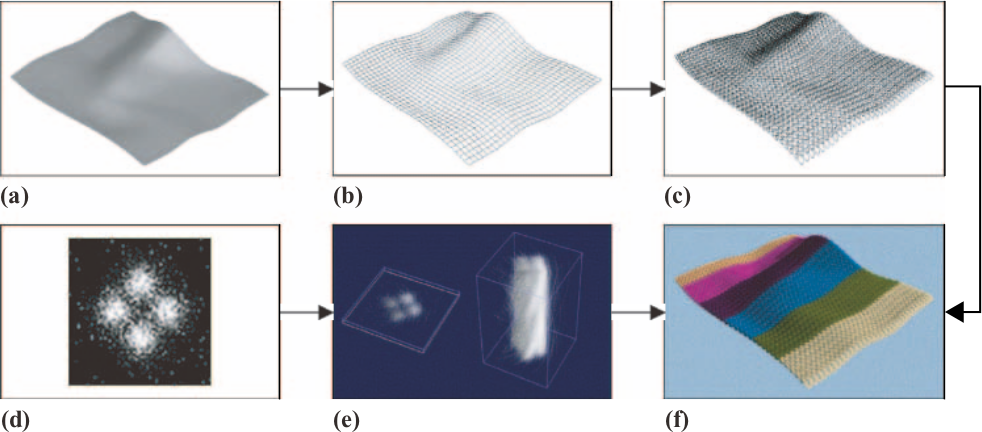
\includegraphics[width=13cm]{figures/tela}
\caption{Pasos para la definición de un modelo de una tela, donde se toman en cuenta fibras individuales. Además de la utilización de una superficie (a), la misma se subdivide (b) para alojar distintas estructuras de hilo (c), los cuales se modelan individualmente ((d) y (e)).}
\label{fg:tela}
\end{figure}

\subsection{Pinturas de autos}
Determinadas marcas de automotores han presentado la necesidad de una correcta visualización de pinturas.
Las mismas se han utlizado para mostrar autos nuevos, o permitir a los posibles compradores jugar con colores y características deseadas para las pinturas.
Debido a esto, es deseable un buen modelo del material en computación gráfica, que permita luego una reproducción lo más fiel posible del mismo en la realidad.

Se han desarrollado principalmente dos métodos para obtener un material en computación gráfica con la apariencia de una pintura de automóviles: basado en primeros principios \cite{Ershov2001}, y basado en medidas de pinturas reales.

En el primero se realiza un modelo por capas, donde cada capa contiene partículas de pigmentos como en las pinturas reales.
El modelo de dos capas presentados asume una capa con partículas que reflejan la luz como un espejo, y la otra con una pintura opaca.
Tomando en consideración parámetros como la densidad, la distrbución de las orientaciones de las partículas, la transmitancia y la reflectancia, derivan una compleja BRDF parametrizada y analítica que permite definir distintos tipos de pinturas, ver Fig.~\ref{fg:pinturaauto}.

En el caso de datos mesurados, es posible utilizar distintas tomas de la reflectancia saliente la pintura de autos para combinarlas en un modelo.
En \cite{Dumont2001} además se utilizan texturas que representan la microgeometría de las pinturas También se utilizó ruido para producir efectos como el denominado {\em brillo} (sparkle).
En otro trabajo \cite{Gunther2005}, se utilizaron los datos de las medidas para producir un modelo analítico estadístico del brillo.
Como puede verse, es posible utilizar diversas metodologías para producir el mismo material o el mismo efecto.
La elección final se hace en base a la complejidad de la captura, costos computacionales, objetivos, y el realismo resultante, entre otros factores.

\begin{figure}
\center
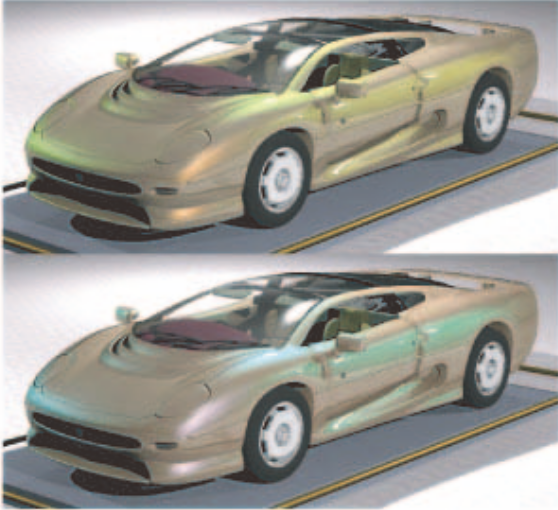
\includegraphics[width=8cm]{figures/pinturaauto}
\caption{Pinturas de autos diseñadas utilizando primeros principios en \cite{Ershov2001}. Cambiando un parámetro pueden obtenerse diferentes apariencias (en este caso, el ancho de las capas de interferencia).}
\label{fg:pinturaauto}
\end{figure}
%\subsection{Fuego}
%\subsection{Humo}

%\subsection{Otros}


\section{Conclusiones}

